\documentclass{beamer}


%----------------------- Preamble ----------------

\usepackage[T1]{fontenc}	%Fremmedord
\usepackage[utf8]{inputenc} %Input type
\usepackage[danish]{babel}	%sprog
\usepackage{lmodern}		%Dansk skriftpakke
\hypersetup{pdfstartview={Fit}}

%Standard sti at søge efter billeder
%--------------------------------------------------
%\begin{figure}[hbtp]
%\centering
%\includegraphics[scale=1]{filnavn-for-png}
%\caption{Titel}
%\label{fig:referenceNavn}
%\end{figure}
%--------------------------------------------------
\usepackage{graphicx}
\usepackage{float}
\graphicspath{{Figurer/}}


%Speciel skrift for enkelt linje kode
%--------------------------------------------------
%Udskriver med fonten 'Courier'
%Mere info her: http://tex.stackexchange.com/questions/25249/how-do-i-use-a-particular-font-for-a-small-section-of-text-in-my-document
%Eksempel: Funktionen \code{void Hello()} giver et output
%--------------------------------------------------
\newcommand{\code}[1]{{\fontfamily{pcr}\selectfont #1}}

%Tables
%----------------------------------------------------------
\usepackage{tabularx}
\usepackage{multirow} 
\usepackage{multicol} 
\usepackage{booktabs}


\title{ITONK eksamen}
\subtitle{DNS}

\author % (optional, for multiple authors)
{Rasmus Bækgaard\inst{1}}

\institute%[Universitäten Hier und Dort] % (optional)
{
  \inst{1}%
  Information og Kommunikationsteknologi\\
  Ingeniørhøjskolen i Aarhus
}

\date{\today}

\subject{subject\dots}

%----------------------- Preamble ----------------

\begin{document}

	\frame{\titlepage}
	
%\AtBeginSection[]
%{
	\begin{frame}
		\frametitle{Table of content}
		\tableofcontents%[currentsection, currentsubsection]
	\end{frame}
%}

\section{The purpose of DNS}
	\begin{frame}
		\frametitle{What is the purpose of DNS}
		
		
			\begin{itemize}
			\item HLT's replacement in 1982
			\item Phone book
			
				\begin{itemize}
				\item Ask for name -- receive IP-address
				\item Connect directly to IP-address
				\end{itemize}
			
			\end{itemize}
		
	\end{frame}
	
\section{DNS hierarchy}
	\begin{frame}
		\frametitle{DNS hierarchy}
		
		\begin{figure}[hbtp]
		\centering
		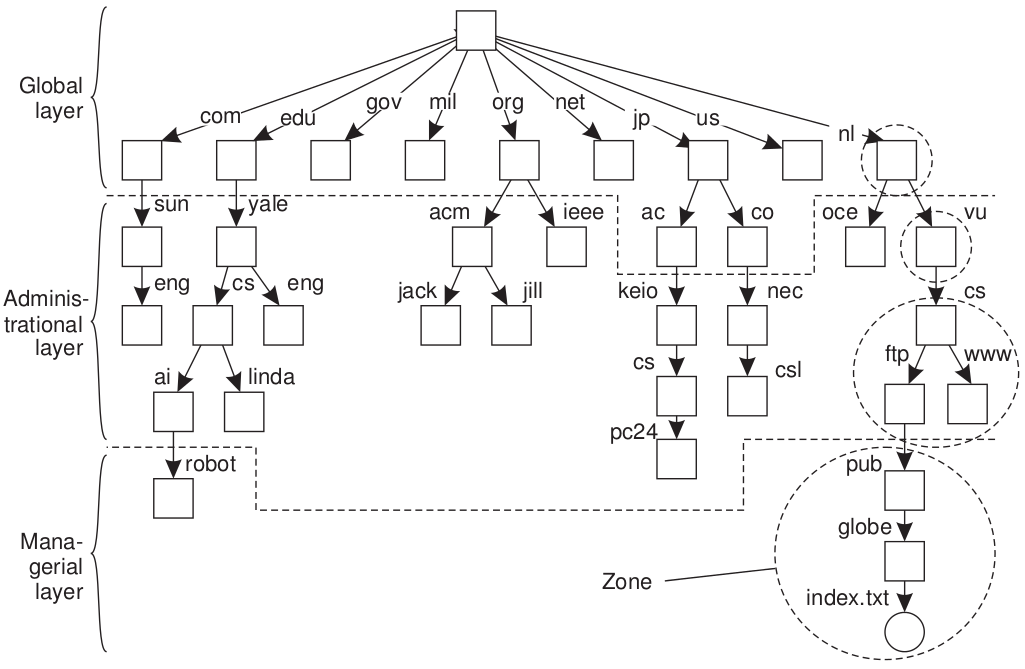
\includegraphics[scale=0.4]{DNS-hierarki}
		\end{figure}
	\end{frame}
	
	
\section{Name resolution}
	\begin{frame}
		\frametitle{Name Resolution}
		
			\begin{itemize}
			\item Iterative name resolution
			\item[]
			\item Recursive name resolution
			%\item Optimal use
			\end{itemize}
		
	\end{frame}
	
\subsection{Iterative name resolution}
	\begin{frame}
		\frametitle{Iterative name resolution}
		
		\begin{figure}[hbtp]
		\centering
		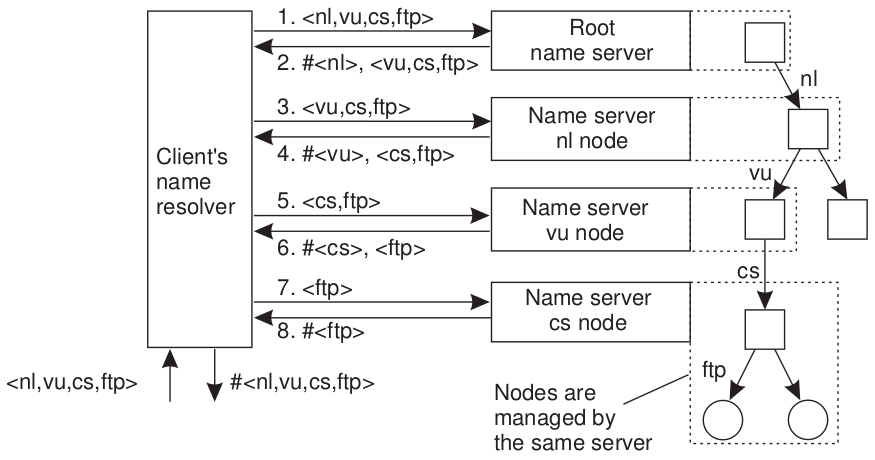
\includegraphics[scale=0.45]{iterativ}
		\end{figure}
		
		
			\begin{itemize}
			\item Notice the '\#' at the response
			\end{itemize}
		
		
	\end{frame}
	

\subsection{Recursive name resolution}
	\begin{frame}
		\frametitle{Recursive name resolution}
		
		\begin{figure}[hbtp]
		\centering
		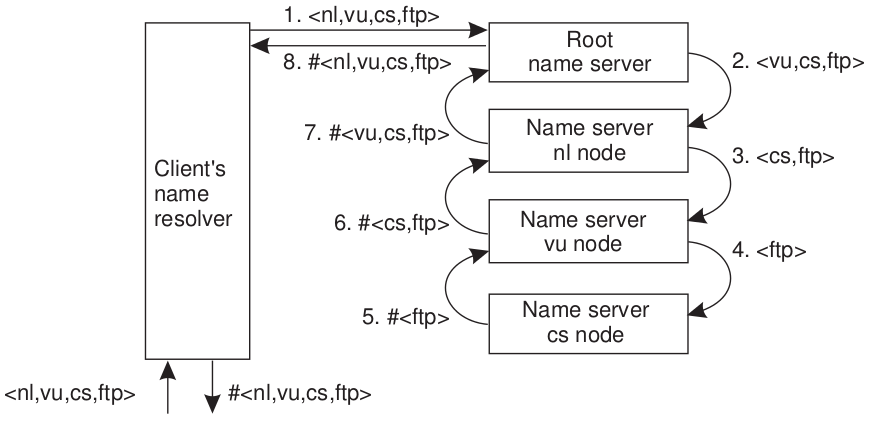
\includegraphics[scale=0.45]{recursiv}
		\end{figure}		
		
	\end{frame}
	
	
\section{BIND, caching and forwarder}
	\begin{frame}
		\frametitle{BIND, caching and forwarder}
		
			\begin{itemize}
			\item Berkeley Internet Name Domain %Univeritet i Californien 
			\item Written 1984 -- rewritten 1985
			\item Caching of requests (\code{dig www.iha.dk})
			\item Forwarding / filter
			\end{itemize}
			
			\begin{figure}[H]
				\begin{minipage}[b]{0.45\linewidth}
				\centering
				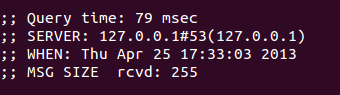
\includegraphics[width=\linewidth]{dig1}
				\caption{\code{dig 127.0.0.1} first time}
				\end{minipage}			
				\hspace{0.5cm}
				\begin{minipage}[b]{0.45\linewidth}
				\centering
				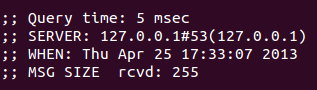
\includegraphics[width=\linewidth]{dig2}
				\caption{\code{dig 127.0.0.1} second time}
				\end{minipage}
			\end{figure}
		
	\end{frame}
	
	
	
\section{DNS Security Extention}
	\begin{frame}
		\frametitle{DNS Security Extention (DNSSEC)}
		
		
			\begin{itemize}
			\item DNS has no security -- as it is.
			\item Signed zone -- trust anchor.
			\item Private key (local) encrypts with public key (server)
			\end{itemize}
			
			\begin{figure}[hbtp]
			\centering
			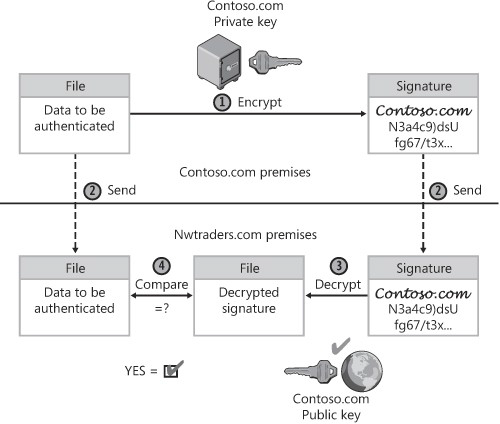
\includegraphics[scale=0.5]{keys}
			\end{figure}
		
		
	\end{frame}
	
%
%\section{some content}
%  \begin{frame}
%    \frametitle{Architecture}
%    
%	\begin{itemize}
%	\item RMI architecture contains three layers
%	
%		\begin{itemize}
%		\item Sub/Skeleton -- also called proxy layer
%		
%			\begin{itemize}
%			\item Closest to client
%			\end{itemize}
%	
%		\item Remote reference
%		\item Transport layer
%		
%		\end{itemize}
%	
%	\end{itemize}
%
%  \end{frame}
%
%  
%\subsection{Design}
%  \begin{frame}
%    \frametitle{Design}
%	
%		\begin{itemize}
%		\item Remote interface
%		
%			\begin{itemize}
%			\item Clients program to remote interfaces
%			\end{itemize}
%		
%		\item Serialization \\
%		 Ved kommunikationen skal der serialiseres
%		\item RMI registry
%		
%		\end{itemize}
%	
%  \end{frame}
%
% 
% 
%\section{some content}
%  \begin{frame}
%    \frametitle{Architecture}
%    
%	\begin{itemize}
%	\item RMI architecture contains three layers
%	
%		\begin{itemize}
%		\item Sub/Skeleton -- also called proxy layer
%		
%			\begin{itemize}
%			\item Closest to client
%			\end{itemize}
%	
%		\item Remote reference
%		\item Transport layer
%		
%		\end{itemize}
%	
%	\end{itemize}
%
%  \end{frame}
 
 
\end{document}